\subsection{Spændingsforsyning}
For at opfylde kravene, der er specificeret i \autoref{sec:krav_spaending}, vælges det at benytte en færdigudviklet komponent, der fungerer som en spændingsregulator. 
Denne benytter to $1,5~V$'s AA-batterier som forsyning. 
Batteriernes kobling danner en split supply. 
Da batterierne sidder i serie, har systemet en positiv spændingsforsyning, ${V}_{cc}$, og en negativ spændingsforsyning, ${V}_{dd}$. 
Jordforbindelsen tages således fra tilslutningen mellem de to batterier.

Spændingsregulatoren sørger for at levere en konstant spænding på henholdsvis $3,4~V$ og $\pm 5,5~V$.
%\fxnote{Dette gøres ved, at spændingsregulatoren oplagrer spænding fra de to tilkoblede batterier i spoler, når switchfunktionen lukkes. Switchfunktionen åbnes, når spolerne er mættede og en spænding ledes videre i kredsløbet via en diode. Denne switchfunktion åbner og lukker skiftevis i kort tid, hvilket resulterer i, at en konstant spænding ledes til systemet hele tiden.} 
Når batterierne aflades, vil spændingsregulatoren på et tidspunkt ikke være i stand til at opretholde en konstant spænding. 
Dette vil indikeres ved, at en LED vil blinke. 
Yderligere vil LED'en stoppe med at lyse, når batterierne er helt afladede. 
Konfigurationen af spændingsforsyningen fremgår af \autoref{fig:spaendingsforsyning}, hvor terminalerne for $\pm 5,5~V$ fremgår som rød (V+) og blå (V-) og grå (Gnd), mens der på den modsatte side fremgår terminalerne for $3,4~V$ som grøn (Vcc) og grå (Gnd). 

\begin{figure}[H]
\centering
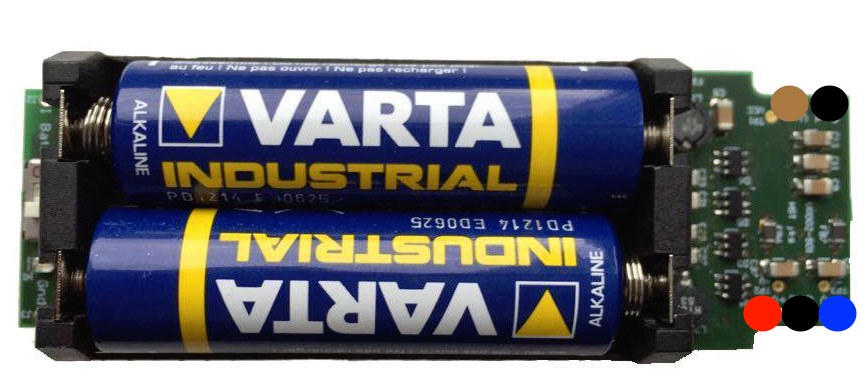
\includegraphics[width=0.6\textwidth]{figures/spaendingsforsyning}
\caption{Spændingsforsyningsregulatoren forsynes af to AA-batterier. Single supply indikeres øverst og illustreres af den grønne (Vcc) og grå prik (Gnd). Split supply indikeres nederst og illustreres af den røde (V+), den blå (V-) og den grå prik (Gnd).}
\label{fig:spaendingsforsyning}
\end{figure}

